\documentclass[12pt]{article}

\usepackage[T1]{fontenc}
\usepackage[margin=1in]{geometry}
\usepackage{xcolor}
\usepackage{tikz}
\usepackage{lmodern}
\usepackage{setspace}
\usepackage{array}
\usepackage{subcaption}
\usepackage{graphicx}
\graphicspath{{figures/}{../figures/}}
\setstretch{1.1}
\usepackage{tikz-3dplot}
\usetikzlibrary{calc}
\usepackage{pgfplots}
\pgfplotsset{compat=1.18}
\usepackage{pgf}
\usepackage{amsmath,amssymb,amsfonts,bm}
\usepgfplotslibrary{fillbetween}
\usepackage[colorlinks=true,linkcolor=blue,citecolor=blue,urlcolor=blue]{hyperref}
\usetikzlibrary{calc}
\definecolor{oiPurple}{RGB}{204,121,167}
\definecolor{oiOrange}{RGB}{230,159,0}
\usepackage{booktabs}
\usepackage{tabularx}
\newcolumntype{L}{>{\raggedright\arraybackslash}X}
\usepackage[numbers,sort&compress]{natbib}
% if you want PRB-like superscripts instead:
\setcitestyle{super,comma,numbers,sort&compress}
% Assumes: graphicx, subcaption are loaded.
% Optional: keep this helper so the PDF shows visible placeholders before images exist.
\newcommand{\maybeinclude}[2][]{%
  \IfFileExists{#2}{\includegraphics[#1]{#2}}{%
    \fbox{\begin{minipage}[c][0.22\textheight][c]{0.95\linewidth}
      \centering\small PLACEHOLDER\\\texttt{#2}
    \end{minipage}}%
  }%
}

% preamble (once)
\usepackage{subcaption}
\usepackage{tikz}

% fixed panel geometry (tune \panelh if needed)
\newlength{\panelw}
\newlength{\panelh}
\setlength{\panelw}{0.30\textwidth}
\setlength{\panelh}{6cm} % all six panels get the same height

% helper (once): same-size box + label inside bottom-right
\newcommand{\panelin}[2]{% #1=(a)... #2=file
  \begin{tikzpicture}
    \node[inner sep=0, outer sep=0] (box) {%
      \begin{minipage}[c][\panelh][c]{\linewidth}
        \centering
        \includegraphics[width=\linewidth,height=\panelh,keepaspectratio]{#2}%
      \end{minipage}%
    };
    \node[anchor=south east, xshift=-1.2mm, yshift=1.2mm] at (box.south east)
      {\footnotesize\textbf{#1}};
  \end{tikzpicture}%
}

% ------------ figure toggles (all OFF by default) ------------
\newif\ifshowIntroGridFigure      % intro 2x3 figure
\newif\ifshowGeometryFigures      % system + sample geometry
\newif\ifshowMosaicTwoDFigure     % mosaic_2d cross-section
\newif\ifshowPvArcFigure          % pv_arc kernel
\newif\ifshowMosaicThreeDFigure   % 3D Bragg-sphere mosaics

\showIntroGridFiguretrue
\showGeometryFigurestrue
\showMosaicTwoDFiguretrue
\showPvArcFiguretrue
\showMosaicThreeDFigurefalse

\begin{document}

\title{Two-dimensional powder diffraction in layered van der Waals films:\\
quantitative X-ray area-detector modeling}
\author{Draft outline}
\maketitle

\section{Introduction}
Layered van der Waals solids are attractive thin-film materials because weak interlayer bonding enables exfoliation, heterostructure assembly, and growth on diverse substrates, while their electronic and transport properties remain sensitive to orientation and stacking.\cite{GeimGrigorieva2013,Jerng2013,Zhang2022Bi2Te3} Their structure is commonly measured with X-ray reflectivity, diffraction, and area-detector WAXS.\cite{Parratt1954,AlsNielsenMcMorrow2001,SmilgiesBlasini2007,Hexemer2015,Savikhin2020} Depending on the substrate and growth conditions, the layer normals may align with the film normal while the crystallites remain nearly random in in-plane azimuth.\cite{Zhang2022Bi2Te3} This uniaxially textured state is commonly called a two-dimensional (2D) powder: individual crystallites remain three-dimensional, but one crystallographic axis is preferentially aligned.\cite{Kaganer1999,Fischer2023MOFGIWAXS} At a single incidence angle, an area detector records Bragg peaks and diffuse intensity at the same time. These features provide complementary information about the film structure.\cite{SmilgiesBlasini2007,Hexemer2015,Savikhin2020}

Figure~\ref{fig:intro_2x3} illustrates this alignment and places the 2D-powder state between the single-crystal and 3D-powder limits in real, reciprocal, and detector space.

\begin{figure}[H]
  \centering
  \captionsetup{font=footnotesize}
  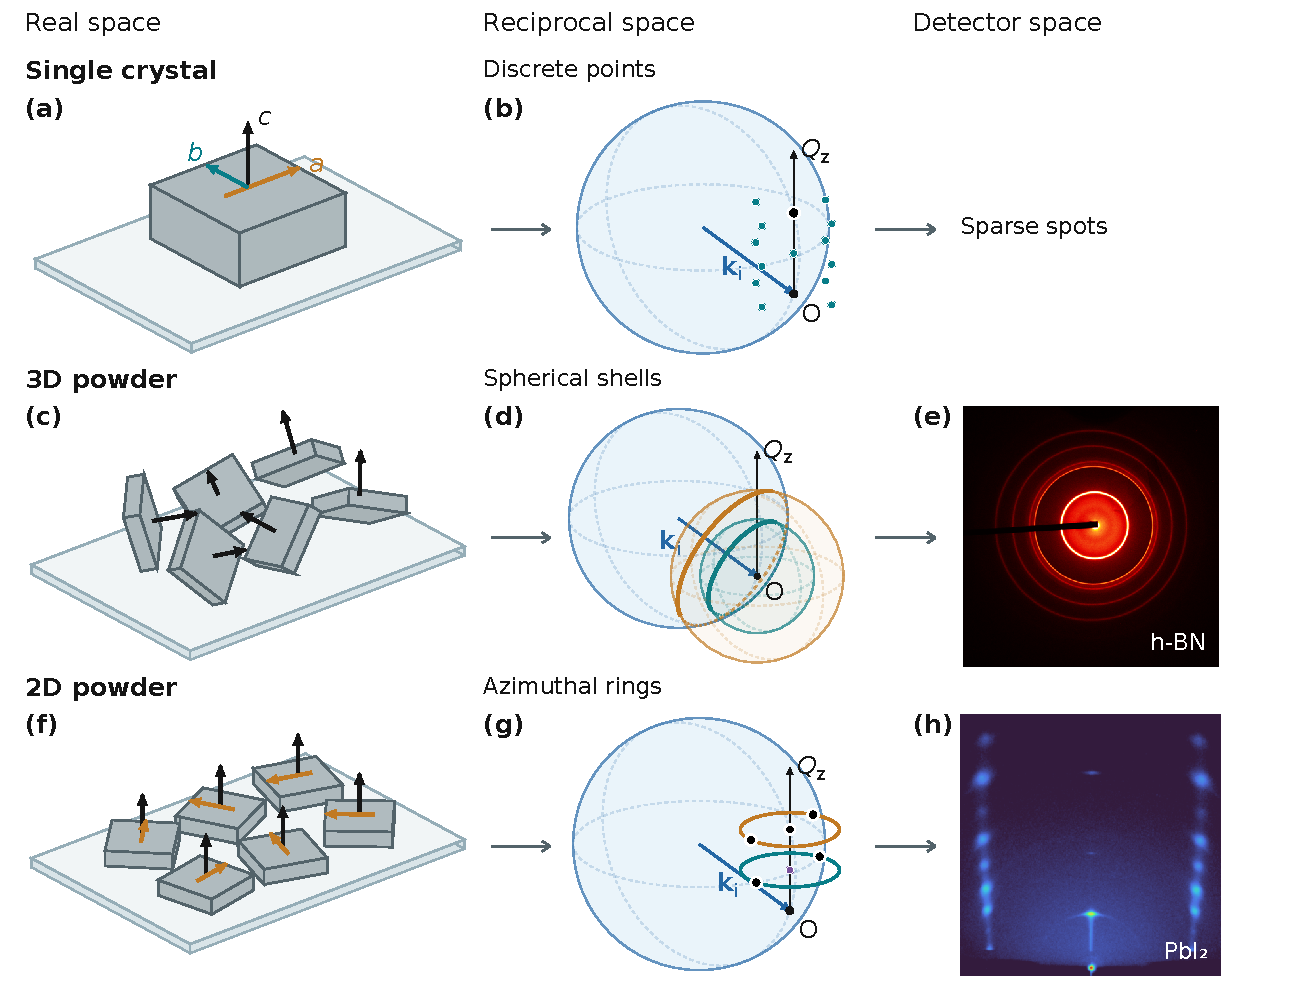
\includegraphics[width=\linewidth]{figures/intro/orientational_limits_reference_journal.pdf}
  \caption[Diffraction across three orientational limits]{Crystallite orientation controls the reciprocal-space distribution and resulting detector pattern. A single crystal gives discrete reciprocal-lattice points (a,b). Random three-dimensional orientations give spherical shells (c,d) and Debye--Scherrer rings, illustrated by h-BN (e). A common film normal with random in-plane azimuth gives off-axis reciprocal-space rings (f,g), whose Ewald intersections produce paired off-specular features, illustrated by PbI$_2$ (h). Arrows between columns indicate this correspondence. Black real-space arrows mark crystallite normals, orange arrows mark an in-plane direction, and $a,b,c$ label crystal axes. Blue spheres show the Ewald construction, with incident wavevector $\mathbf{k}_i$, reciprocal origin $O$, and film-normal axis $Q_z$. Teal and orange distinguish reflection loci. Black points and thick colored curves mark selected intersections, dashed curves are construction guides, and the purple axial point is unselected.}
  \label{fig:intro_2x3}
\end{figure}

Here $\mathbf{k}_i$ and $\mathbf{k}_f$ are the incident and exit wavevectors, and $\mathbf Q=\mathbf{k}_f-\mathbf{k}_i$ is the momentum transfer. The Ewald sphere is centered at $-\mathbf{k}_i$, passes through the reciprocal-space origin, and has radius $|\mathbf{k}_i|=2\pi/\lambda$. Elastic diffraction selects reciprocal-space intensity satisfying $|\mathbf{k}_i+\mathbf Q|=|\mathbf{k}_i|$, and each selected $\mathbf Q$ defines $\mathbf{k}_f=\mathbf{k}_i+\mathbf Q$.\cite{AlsNielsenMcMorrow2001} A single crystal supplies isolated reciprocal-lattice points, while random 3D orientations spread each reflection over a spherical shell. In a 2D powder, random in-plane azimuth spreads each off-axis reflection into a ring about the film-normal reciprocal-space axis, while $(00L)$ intensity remains near that axis.\cite{Kaganer1999,SmilgiesBlasini2007} The Ewald sphere generally intersects an off-axis ring at two points, which map to paired detector features.\cite{SmilgiesBlasini2007,Hexemer2015,Smilgies2005Rods} Mosaicity and other experimental effects broaden these ideal intersections into arcs and cap-like intensity while preserving the same elastic condition.

Figure~\ref{fig:area_detector_overview} shows a representative measured PbI$_2$ pattern.

\begin{figure}[H]
  \centering
  \captionsetup{font=footnotesize}
  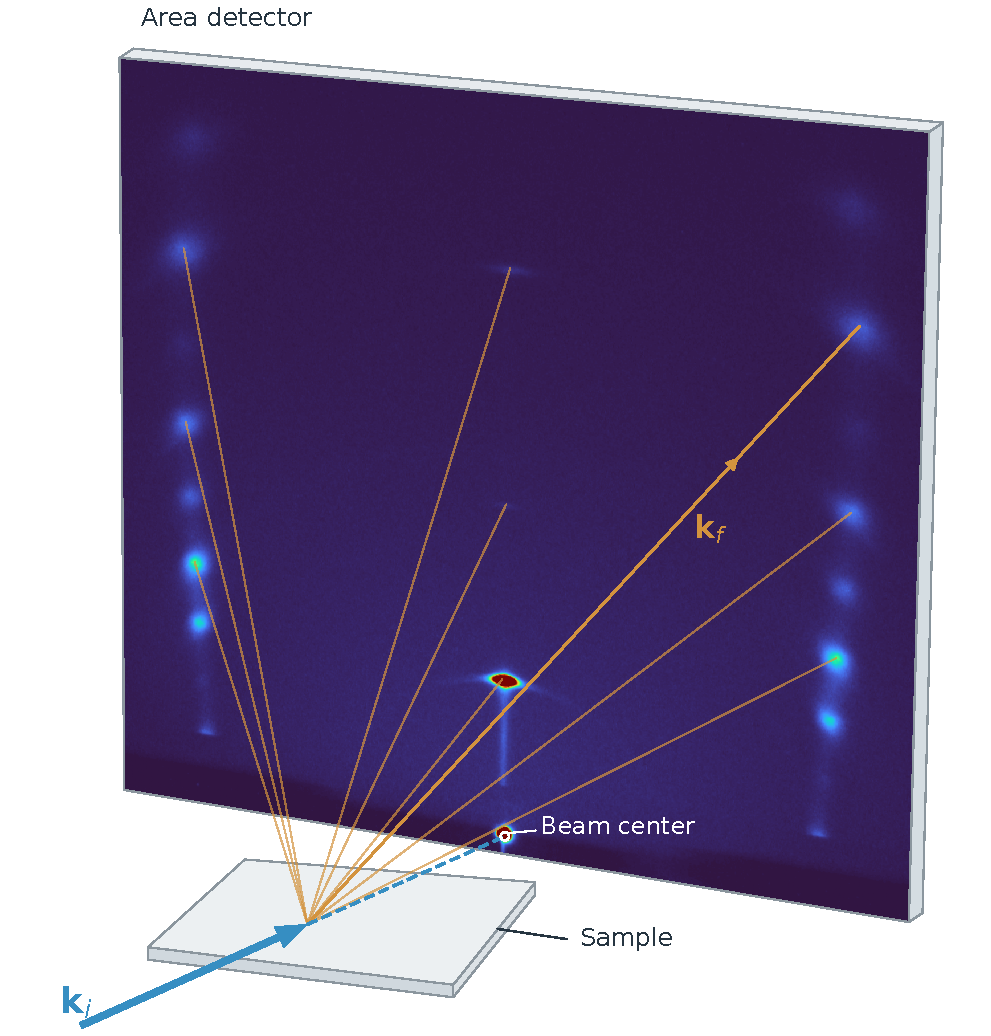
\includegraphics[width=0.62\linewidth]{figures/intro/area_detector_overview_journal.pdf}
  \caption[Area-detector measurement of a 2D powder]{An area detector records multiple diffraction features simultaneously, at positions displaced from the undeflected-beam reference. The displayed pattern is measured from a PbI$_2$ film. The blue arrow marks the incident wavevector $\mathbf{k}_i$, and its dashed continuation reaches the beam center, marked by an open circle. Orange rays connect the sample to selected diffraction features, with one scattered wavevector $\mathbf{k}_f$ identified by an arrowhead. Peaks, arcs, and intensity between peaks are recorded in the same exposure.}
  \label{fig:area_detector_overview}
\end{figure}

Standard WAXS workflows often integrate area-detector images into one-dimensional profiles, an effective representation for nearly isotropic powders.\cite{Ashiotis2015,Hexemer2015,Savikhin2020,Reus2024} For a 2D powder, retaining the radial and transverse detector directions keeps the specular and off-specular features as separate, complementary constraints. Stacking disorder is also commonly treated with one-dimensional interference models.\cite{HendricksTeller1942,Treacy1991,CasasCabanas2016} Full orientation-distribution-function refinements can represent arbitrary textures,\cite{WenkVanHoutte2004,Lutterotti2004TSF,VonDreele1997,LutterottiVasinWenk2014} while more constrained cases can be represented by lower-dimensional preferred-orientation kernels\cite{March1932,Dollase1986} or a small number of epitaxial variants.\cite{Smilgies2000POPOP} The present work considers the 2D-powder limit. The approximately azimuthally symmetric measured features motivate axial symmetry about the film normal and a compact out-of-plane mosaicity distribution. We therefore use the off-specular arcs and axial-family profiles as complementary constraints on the same orientation model.

The optical boundary conditions follow established grazing-incidence formalisms,\cite{Sinha1988,Renaud2009,Hexemer2015,Savikhin2020} while the reciprocal-rod geometry and allowed-reflection locations build on reciprocal-space mapping and detector-space indexing for oriented films.\cite{SmilgiesBlasini2007,Smilgies2005Rods,Breiby2008,SmilgiesLi2026IndexGIXS} For these data, wavelength bandwidth, beam divergence, refraction, sample misalignment, mosaicity, and stacking disorder can redistribute intensity in overlapping ways. We therefore evaluate them within one calculation.
Source position and divergence are sampled from the measured Gaussian beam distributions, while wavelength is sampled from the input wavelength spectrum. For each $\mathbf{k}_i$, the model constructs a structure function, applies the corresponding Ewald condition, and maps the accepted intensity to the calibrated detector. The forward calculation incorporates these corrections. Applying identical integration regions to the measured and calculated detector intensities preserves the radial and transverse information.

Figures~\ref{fig:ordered_bi2se3_test} and~\ref{fig:ordered_bi2te3_test} present the Bi$_2$Se$_3$ and Bi$_2$Te$_3$ detector comparisons and selected profiles at nominal $5^\circ$ incidence, a condition included in the refinement. The panels separate the off-axis rod families from the axial response. These ordered-film test cases are followed by the staged refinement workflow and then the PbI$_2$ stacking-disorder extension.

\section{Diffraction Model}
\label{sec:diffraction_model}
We refer to the model as a forward model because it follows the physical sequence from ray to sample to detector. The incident beam on the sample is represented by weighted source states sampled in position, direction, and wavelength. Each incident ray is described by its incident angles $(\theta_i,\phi_i)$ and wavevector magnitude $|\mathbf{k}_i|=2\pi/\lambda$, so its state is written as $\mathbf{k}_i(|\mathbf{k}_i|,\theta_i,\phi_i)$. Sample composition and crystallinity determine a reciprocal-space structure function $S(\mathbf{k}_i,\mathbf Q)$. Restricting this density to the Ewald sphere defined by $\mathbf{k}_i$ produces an Ewald surface decorated by the intensities in $\mathbf{Q}$. The corresponding $\mathbf{k}_f$ vectors carry the selected intensities toward the shared geometry of the chosen X-ray collection method, namely a 2D area detector.

\subsection{Scattering and detector geometry}
\label{sec:scattering_detector_geometry}
For one incident state, let $\mathbf{k}_i$ denote the incident wavevector and $\mathbf{k}_f$ the scattered wavevector. For wavelength $\lambda$, elastic scattering preserves their magnitudes,
\begin{equation}
  |\mathbf{k}_i|=|\mathbf{k}_f|=\frac{2\pi}{\lambda}.
  \label{eq:elastic_scattering}
\end{equation}
The momentum transfer is
\begin{equation}
  \mathbf Q=\mathbf{k}_f-\mathbf{k}_i.
  \label{eq:momentum_transfer}
\end{equation}
For an infinite, perfectly ordered crystal, an allowed reflection $(h,k,\ell)$ supplies
\begin{equation}
  \mathbf G_{hk\ell}=h\mathbf a^{*}+k\mathbf b^{*}+\ell\mathbf c^{*},
  \qquad \mathbf Q=\mathbf G_{hk\ell},
  \label{eq:bragg_matching}
\end{equation}
where $\mathbf a^{*}$, $\mathbf b^{*}$, and $\mathbf c^{*}$ include the factor $2\pi$. The corresponding exit wavevector is
\begin{equation}
  \mathbf{k}_f=\mathbf{k}_i+\mathbf G_{hk\ell}.
  \label{eq:exit_wavevector}
\end{equation}
Equations~\eqref{eq:bragg_matching} and~\eqref{eq:exit_wavevector} define the ideal integer Bragg-point limit. Replacing the integer order $\ell$ by a continuous coordinate $L$ generalizes the same construction to a reciprocal rod, with the Bragg orders lying at $L=\ell$.

Figure~\ref{fig:waxs_geometry_system} shows how an accepted exit direction reaches the area detector. In the laboratory frame, $y$ follows the nominal incident beam, $z$ is vertical, and $x$ is transverse. The scattering angle $2\theta$ is the angle between $\mathbf{k}_i$ and $\mathbf{k}_f$. The outgoing-ray azimuth $\phi_f$ is measured about the incident direction, with zero toward $+z$ in the reference geometry.

The detector axes $x'$ and $z'$ lie in its plane, and $\hat{\mathbf n}_{\mathrm{det}}$ points out of its active face toward the sample. The nominal sample-to-detector distance $D$ is measured along the beam axis in the untilted reference geometry. Detector tilts $\beta_D$ and $\gamma_D$ change the plane orientation. Supporting Information Sec.~S1 gives the corresponding detector-frame coordinates, signed angular convention, and ray--plane intersection equations.

\begin{figure}[H]
  \centering
  \resizebox{0.6\linewidth}{!}{% Detector geometry TikZ figure (to be \input into main document)

\tdplotsetmaincoords{70}{120}
\begin{tikzpicture}[tdplot_main_coords, scale=1.5]

    %=========================
    % Parameters
    %=========================
    % Geometry angles (keep detector unrotated)
    \pgfmathsetmacro{\alpha}{0}         % detector tilt about x (deg)
    \pgfmathsetmacro{\betaang}{0}       % detector rotation about z (deg)

    % Display-only angles (nonzero annotations)
    \pgfmathsetmacro{\betaVis}{-20}      % shown beta angle (deg)
    \pgfmathsetmacro{\gammaVis}{20}     % shown gamma angle (deg)

    \pgfmathsetmacro{\detW}{2}           % detector width
    \pgfmathsetmacro{\detH}{2}           % detector height
    \pgfmathsetmacro{\detT}{0.2}         % detector thickness

    \pgfmathsetmacro{\detHw}{0.5*\detW}  % half-width
    \pgfmathsetmacro{\detHh}{0.5*\detH}  % half-height

    % Geometry sines and cosines
    \pgfmathsetmacro{\sina}{sin(\alpha)}
    \pgfmathsetmacro{\cosa}{cos(\alpha)}
    \pgfmathsetmacro{\sinb}{sin(\betaang)}
    \pgfmathsetmacro{\cosb}{cos(\betaang)}

    % Display trig
    \pgfmathsetmacro{\sinBetaVis}{sin(\betaVis)}
    \pgfmathsetmacro{\cosBetaVis}{cos(\betaVis)}
    \pgfmathsetmacro{\sinGammaVis}{sin(\gammaVis)}
    \pgfmathsetmacro{\cosGammaVis}{cos(\gammaVis)}

    % Detector center (front face)
    \coordinate (detCenter) at (-3,0,0);

    %=========================
    % Detector local basis (tilt about x then rotation about z)
    %=========================
    % Horizontal (width) direction
    \coordinate (detU) at ({-\detHw*\sinb},{\detHw*\cosb},0);

    % Vertical (height) direction
    \coordinate (detV) at ({\detHh*\sina*\cosb},
                           {\detHh*\sina*\sinb},
                           {\detHh*\cosa});

    % Thickness direction (front to back)
    \coordinate (detTvec) at ({-\detT*\cosa*\cosb},
                              {-\detT*\cosa*\sinb},
                              {\detT*\sina});

    % Components of detV for use in arc centers
    \pgfmathsetmacro{\Vx}{\detHh*\sina*\cosb}
    \pgfmathsetmacro{\Vy}{\detHh*\sina*\sinb}
    \pgfmathsetmacro{\Vz}{\detHh*\cosa}

    % Bottom center coordinates: detFBC = detCenter - detV
    \pgfmathsetmacro{\FBCx}{-3 - \Vx}
    \pgfmathsetmacro{\FBCy}{0  - \Vy}
    \pgfmathsetmacro{\FBCz}{0  - \Vz}

    % Bottom right coordinates: detFBR = detCenter + detU - detV
    \pgfmathsetmacro{\FBRx}{-3 - \detHw*\sinb - \Vx}
    \pgfmathsetmacro{\FBRy}{    \detHw*\cosb - \Vy}
    \pgfmathsetmacro{\FBRz}{          0      - \Vz}

    % Top right coordinates: detFTR = detFBR + 2*detV
    \pgfmathsetmacro{\FTRx}{\FBRx + 2*\Vx}
    \pgfmathsetmacro{\FTRy}{\FBRy + 2*\Vy}
    \pgfmathsetmacro{\FTRz}{\FBRz + 2*\Vz}

    %=========================
    % Detector bottom-center point
    %=========================
    \coordinate (detFBC) at ({\FBCx},{\FBCy},{\FBCz});

    %=========================
    % Detector geometry
    %=========================
    % Front face corners
    \coordinate (detFBL) at ($ (detCenter) - (detU) - (detV) $); % bottom left
    \coordinate (detFBR) at ($ (detCenter) + (detU) - (detV) $); % bottom right
    \coordinate (detFTL) at ($ (detCenter) - (detU) + (detV) $); % top left
    \coordinate (detFTR) at ($ (detCenter) + (detU) + (detV) $); % top right

    % Back face corners
    \coordinate (detBBL) at ($ (detFBL) + (detTvec) $);
    \coordinate (detBBR) at ($ (detFBR) + (detTvec) $);
    \coordinate (detBTL) at ($ (detFTL) + (detTvec) $);
    \coordinate (detBTR) at ($ (detFTR) + (detTvec) $);

    % Hidden-edge style
    \tikzset{
      detectorHidden/.style={
        line width=0.45pt,
        dashed,
        dash pattern=on 2pt off 1.2pt
      }
    }

    % Draw back face edge-by-edge
    \draw[detectorHidden] (detBBL) -- (detBBR); % bottom back
    \draw[very thick]     (detBBR) -- (detBTR); % right back
    \draw[very thick]     (detBTR) -- (detBTL); % top back
    \draw[detectorHidden] (detBTL) -- (detBBL); % left back

    % Draw front face
    \draw[very thick]
      (detFBL) -- (detFBR) -- (detFTR) -- (detFTL) -- cycle;

    % Connector edges (thickness)
    \draw[very thick]     (detFBR) -- (detBBR);
    \draw[very thick]     (detFTR) -- (detBTR);
    \draw[very thick]     (detFTL) -- (detBTL);
    \draw[detectorHidden] (detFBL) -- (detBBL);

    % Detector label
    \node at ($(detCenter)+(0,0,1.3)$) {\scriptsize Detector};
    %=========================
    % Detector-frame axes (schematic)
    %=========================
    \draw[->, black, line width=0.2mm] (detCenter) -- ($ (detCenter) + 0.9*(detU) $)
      node[anchor=west, scale=0.5, xshift = -12, yshift = -6] {$x'$};
    \draw[->, black, line width=0.2mm] (detCenter) -- ($ (detCenter) + 0.9*(detV) $)
      node[anchor=south, scale=0.5, xshift = -8, yshift = -20] {$z'$};


% Detector normal anchor point on the front face
\coordinate (detNormalBase) at ($ (detCenter) + 0.55*(detU) - 0.35*(detV) $);
\coordinate (detNormalTip)  at ($ (detNormalBase) - 2.6*(detTvec) $);

% Optional style definitions
\tikzset{
  detNormalArrow/.style={
    ->,
    black,
    line width=0.3mm,
    preaction={draw, white, line width=0.9mm}
  },
  detNormalPoint/.style={
    fill=black,
    draw=white,
    line width=0.25pt
  }
}

% Mark the point on the detector surface
\filldraw[detNormalPoint] (detNormalBase) circle (0.7pt);

% Draw the detector normal with a subtle white halo
\draw[detNormalArrow] (detNormalBase) -- (detNormalTip)
  node[pos=0.92, anchor=north west, scale=0.52,
       xshift=2pt, yshift=-1pt,
       fill=white, inner sep=1pt, text=black]
  {$\hat{n}_{\mathrm{det}}$};
  
    %=========================
    % Beta arc, line, and label at top-right (display-only)
    %=========================
    \pgfmathsetmacro{\rBetaArc}{0.3}
    \pgfmathsetmacro{\betastart}{min(0,\betaVis)}
    \pgfmathsetmacro{\betaend}{max(0,\betaVis)}
    \pgfmathsetmacro{\betamid}{0.5*(\betastart+\betaend)}

    % Dashed line for beta from top-right in a local xz plane
    \coordinate (betaBase) at ({\FTRx},{\FTRy},{\FTRz});
    \coordinate (betaDet) at ({\FTRx + \rBetaArc*\sinBetaVis},
                              {\FTRy},
                              {\FTRz + \rBetaArc*\cosBetaVis});
    \draw[orange, dash pattern=on 1pt off 0.7pt] (betaBase) -- (betaDet);

    % Vertical z bar at top-right
    \coordinate (detFTRzBar) at ($ (detFTR) + (0,0,0.3) $);
    \draw[orange,thick] (detFTR) -- (detFTRzBar);

    % Arc for beta at top-right
    \draw[orange, dash pattern=on 1pt off 0.7pt, line width=0.1mm] 
      plot[domain=\betastart:\betaend, samples=30, variable=\t]
        ({\FTRx + \rBetaArc*sin(\t)},
         {\FTRy},
         {\FTRz + \rBetaArc*cos(\t)});

    % Label for beta at top-right
    \coordinate (betaLabel) at ({\FTRx + 1.1*\rBetaArc*sin(\betamid)},
                                {\FTRy},
                                {\FTRz + 1.1*\rBetaArc*cos(\betamid)});
    \node[orange, scale=0.6, anchor=south east,
          xshift=6pt, yshift=-5pt] at (betaLabel) {$\beta$};

    %=========================
    % Gamma arc, lines, and label at top-right (display-only)
    %=========================
    \pgfmathsetmacro{\rArc}{0.4}
    \pgfmathsetmacro{\alphab}{90+\gammaVis}   % rotated edge direction (display)
    \pgfmathsetmacro{\alphax}{90}             % reference +y
    \pgfmathsetmacro{\alphastart}{min(\alphab,\alphax)}
    \pgfmathsetmacro{\alphaend}{max(\alphab,\alphax)}
    \pgfmathsetmacro{\alphamid}{0.5*(\alphastart+\alphaend)}

    \coordinate (gammaBase) at ({\FTRx},{\FTRy},{\FTRz});
    % display edge direction using (-sin, cos)
    \coordinate (gammaWidthEnd) at ({\FTRx - 0.4*\sinGammaVis},
                                    {\FTRy + 0.4*\cosGammaVis},
                                    {\FTRz});
    % reference +y direction
    \coordinate (gammaXEnd) at ({\FTRx},
                                {\FTRy + 0.4},
                                {\FTRz});
    \draw[oiPurple,thick] (gammaBase) -- (gammaWidthEnd);
    \draw[oiPurple,thin]  (gammaBase) -- (gammaXEnd);

    % Gamma arc centered at top-right
    \draw[oiPurple, line width=0.1mm, dash pattern=on 1pt off 0.7pt]
      plot[domain=\alphastart:\alphaend, samples=30, variable=\t]
        ({\FTRx + \rArc*cos(\t)},
         {\FTRy + \rArc*sin(\t)},
         {\FTRz});

    % Label for gamma
    \coordinate (gammaLabel) at ({\FTRx + 0.7*cos(\alphamid)},
                                 {\FTRy + 0.7*sin(\alphamid)},
                                 {\FTRz});
    \node[oiPurple, scale=0.6, anchor=south west,
          xshift=-18pt, yshift=-5pt] at (gammaLabel) {$\gamma$};

    %=========================
    % Sample and beams
    %=========================
    % Incident beam from sample to detector center
    \draw[black, dash dot] (-0.5,0,0) -- (detCenter);

    % Sample plane
    \draw[fill=gray]
      (-0.312, -0.2, -0.068) --
      (-0.312,  0.2, -0.068) --
      (-0.688,  0.2,  0.068) --
      (-0.688, -0.2,  0.068) -- cycle;

    \node[scale=0.7, xshift = -15, yshift = 25] at (-0.212, 0.3, -0.088) {\tiny Sample};

    % Incident beam from source to sample
    \draw[black, dash dot] (0.5,0,0) -- (-0.5,0,0);

    %=========================
    % Scattered point and components
    %=========================
    \pgfmathsetmacro{\offY}{0.8}  % along U0 (width)
    \pgfmathsetmacro{\offZ}{0.3}  % along V0 (height)

    \coordinate (scatP) at ({-3 + \offZ*\sina*\cosb - \offY*\sinb},
                            {\offZ*\sina*\sinb + \offY*\cosb},
                            {\offZ*\cosa});

    % Width-component point: detCenter + offY * u_hat, u_hat = (-sinb, cosb, 0)
    \coordinate (scatPwidth) at ({-3 - \offY*\sinb},
                                 {0  + \offY*\cosb},
                                 {0});

    \draw[dash pattern=on 2pt off 1pt, green] (detCenter) -- (scatP);
    \draw[dash pattern=on 2pt off 1pt,green] (detCenter) -- (scatPwidth);
    \draw[dash pattern=on 2pt off 1pt,green] (scatPwidth) -- (scatP);

    % Scattered beam vector r
    \draw[red,->] (-0.5,0,0) -- (scatP);
    \node[scale=0.7, red, xshift=12pt, yshift=-2pt]
      at ($ (-0.5,0,0)!0.6!(scatP) $) {\tiny $\vec{k}_f$};

    % Incident vector k_i
    \draw[blue,->] (0.5,0,0) -- (-0.5,0,0);
    \node[scale=0.7, blue, yshift= -0.5mm] at (0.0,0.12,-0.01) {\tiny $\vec{k}_i$};

    %=========================
    % Angle arcs for phi and 2theta
    %=========================
    \tdplotsetrotatedcoords{0}{90}{90}
    \tdplotdrawarc[dashed,tdplot_rotated_coords, cyan]
      {(0,0,-3)}{0.8}{20}{90}{anchor=north west, xshift = -8pt}{\tiny $\phi$}

    \tdplotsetrotatedcoords{90}{-20.56}{0}
    \tdplotdrawarc[dashed, green,tdplot_rotated_coords, line width=0.1mm]
      {(0,1.4,0)}{0.5}{15}{90}
      {anchor=south east}{\tiny $2\theta$}

    %=========================
    % Axes legend
    %=========================
    \draw[->] (.5,0,0) -- (0.3,0,0)
      node[anchor=south west, xshift=-1.5mm, yshift=-0.8mm] {\tiny $y$};
    \draw[->] (.5,0,0) -- (.5,0.2,0) node[anchor=west] {\scriptsize $x$};
    \draw[->] (.5,0,0) -- (.5,0,0.2) node[anchor=south] {\scriptsize $z$};

\end{tikzpicture}
}
  \caption{Laboratory and detector geometry in the untilted reference pose. The blue incident wavevector $\mathbf{k}_i$ reaches the sample, and the red scattered wavevector $\mathbf{k}_f$ reaches the detector. The dash-dotted line continues the incident direction and defines the reference for $2\theta$. The azimuth $\phi_f$ is measured from $+z'$ about that direction and is negative for the ray shown. Dashed detector-plane lines resolve the hit position along $x'$ and $z'$. The laboratory axes are $x,y,z$, the outward detector normal is $\hat{\mathbf n}_{\mathrm{det}}$, and $D$ marks the nominal sample-to-detector distance.}
  \label{fig:waxs_geometry_system}
\end{figure}

\begingroup
\clubpenalty=10000
Source position and propagation angles arising from divergence are sampled from the measured Gaussian beam distributions, while wavelength is sampled from the input wavelength spectrum. Supporting Information Sec.~S1 defines the weighted source-state construction. The external ray intersects the measured sample geometry, and refraction gives the internal vector $\mathbf{k}'_i$. Accepted exit rays must intersect the front face within the active detector bounds. Sample acceptance and detector acceptance are therefore consecutive geometric restrictions.
\par\endgroup

\subsection{Structure Factor}
\label{sec:structure_factor}
For the hexagonal basal plane, every integer in-plane pair $(h,k)$ belongs to the radial family
\begin{equation}
  r\equiv h^2+hk+k^2,
  \qquad
  Q_R(r)=\frac{4\pi}{\sqrt{3}\,a}\sqrt r.
  \label{eq:hexagonal_family_index}
\end{equation}
Members with the same $r$ have the same in-plane radius. Their amplitudes are evaluated individually, and their intensity contributions are summed to represent scattering from the radial family. The family label is distinct from crystallographic multiplicity, and the explicit sum accounts for multiplicity.

For one $(h,k)$ member, the crystallite-frame reciprocal rod is
\begin{equation}
  \mathbf G_{hk}(L)=h\mathbf a^{*}+k\mathbf b^{*}+L\mathbf c^{*}.
  \label{eq:continuous_reciprocal_rod}
\end{equation}
The indices $h$ and $k$ are integers, while $L$ is continuous. An integer Bragg order $(h,k,\ell)$ lies at $L=\ell$. The wavelength-dependent amplitude along the rod is
\begin{equation}
  F_{hk}(L,\lambda_s)=
  \sum_a o_a f_a\!\left(|\mathbf G_{hk}(L)|,\lambda_s\right)
  T_a\!\left(\mathbf G_{hk}(L)\right)
  \exp\!\left[i\mathbf G_{hk}(L)\cdot\mathbf r_a\right].
  \label{eq:continuous_structure_factor}
\end{equation}
Here $o_a$, $f_a$, $T_a$, and $\mathbf r_a$ are the occupancy, atomic scattering factor, atomic displacement (Debye--Waller) factor, and Cartesian site position.

The complex amplitude $F_{hk}$ is the structural input evaluated along the reference rod. The remaining calculation uses the continuous rod intensity $S_{hk}(L,\lambda_s)$. For an ordered finite film, $S_{hk}$ is constructed from $|F_{hk}|^2$. $S_{hk}(L,\lambda_s)\,dL$ is the integrated structural intensity carried by a small segment of the unrotated $(h,k)$ rod. Supporting Information Sec.~S2 gives the finite-stack construction, displacement conventions, and conversion between densities per $dL$ and per dimensional rod length.

The cylinder construction follows directly from the definition of a 2D powder in Fig.~\ref{fig:intro_2x3}(f--g): the crystallites share a mean film normal but are random in in-plane azimuth. If $\mathbf C$ maps the mean crystallite frame into the sample frame, rotating a point on the rod through azimuth $\beta$ gives
\begin{equation}
  \mathbf Q^{\mathrm{cyl}}_{hk}(\beta,L)
  =\mathbf C\,\mathbf R_{\widehat{\mathbf c}^{\,*}}(\beta)\mathbf G_{hk}(L),
  \qquad 0\leq\beta<2\pi.
  \label{eq:powder_cylinder}
\end{equation}
Thus, every off-axis rod sweeps out a cylinder about the film-normal reciprocal-space axis, while the axial rod remains on the normal axis. Members with the same $r$ share the same geometric cylinder, although their amplitudes are evaluated separately. For off-axis cylinders with $Q_R>0$, distributing a density per dimensional rod length around the circumference introduces $1/[2\pi Q_R(r)]$. For the density per $dL$ used here, the physical cylinder-area conversion additionally contains $1/|\mathbf c^*|$ (Supporting Information Sec.~S2). This construction produces the paired off-specular trajectories in Fig.~\ref{fig:intro_2x3}(h) while leaving axial reciprocal points on the common normal.

\subsection{Mosaicity}
\label{sec:mosaicity}
A two-dimensional powder is already random in in-plane azimuth. Mosaicity adds a distribution of crystallite tilts about the mean film normal. Its role is visible in the measured detector image in Fig.~\ref{fig:hk0_low_l_star}, where it explains features that are otherwise incompatible with a single incident vector and one perfectly aligned crystallite.

Figure~\ref{fig:hk0_low_l_star} shows the $r=0$ region of a Bi$_2$Se$_3$ image collected at the nominal incident angle $\theta_i=5^\circ$. That incident condition places the Ewald intersection near the $003$ condition. Surprisingly, intensity is also visible near the $006$ location, at approximately twice the radial $2\theta$ coordinate of $003$. The $003$ feature is also strongly anisotropic: its long extension follows the radial $2\theta$ direction, whereas its transverse width follows the outgoing-ray azimuth $\phi$.

For the $003$ peak, the transverse $\phi$ width is primarily due to mosaicity, while the radial spread is better explained by wavelength dispersion. As discussed below, the unexpected $006$ intensity motivates testing a broad component in the mosaic distribution. The bright feature near $L=0$ is specular reflectivity, discussed separately in Sec.~\ref{sec:reflectivity}.


\begin{figure}[H]
  \centering
  \textbf{Radial and transverse structure of the Bi$_2$Se$_3$ $r=0$ region}
  \begin{minipage}{0.92\linewidth}
    \centering
    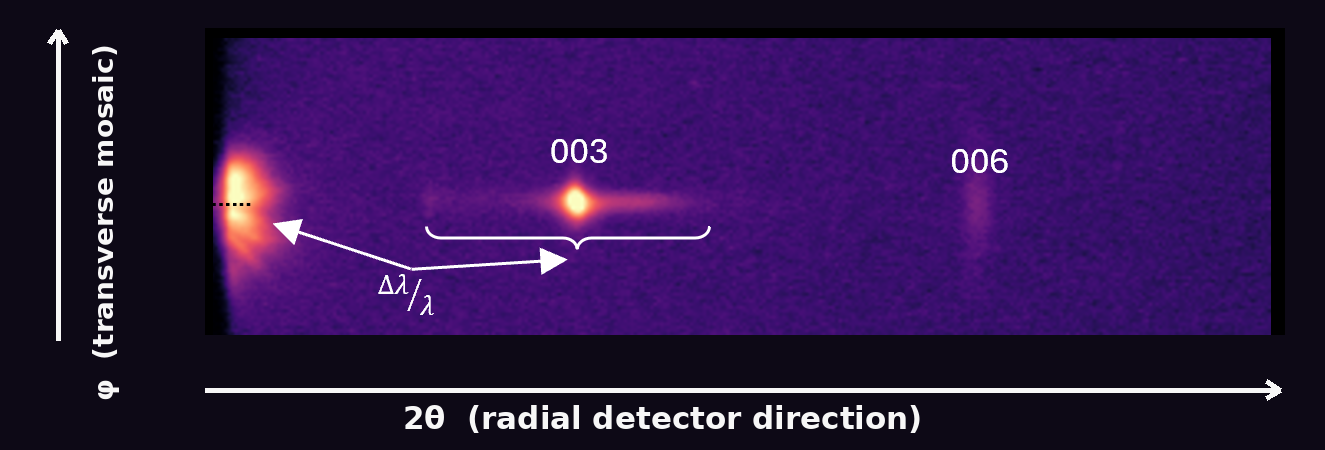
\includegraphics[width=\linewidth]{figures/results_ordered/00L_region_wavelength_mosaic_axes.png}
  \end{minipage}
  \caption{Measured $r=0$ detector region from the $5^\circ$ Bi$_2$Se$_3$ image. The nominal incident condition lies near $003$, while intensity is also observed near the $006$ location at approximately twice its radial $2\theta$ coordinate. The $003$ feature has a long radial extension along $2\theta$, whereas its transverse $\phi$ width is the cleaner constraint on crystallite tilt. The bright near-origin feature is near-critical specular reflectivity discussed in Sec.~\ref{sec:reflectivity}.}
  \label{fig:hk0_low_l_star}
\end{figure}

As shown below, off-specular rod-family arcs and the transverse $\phi$ width of off-condition $r=0$ intensity probe different parts of the same orientation distribution. Strong off-specular arcs mainly constrain crystallites whose normals are close to the mean film normal. Weak $r=0$ intensity farther from the specular direction is more sensitive to the small population at larger tilt.

To apply the crystallite mosaic tilt, we rotate each point on the powder cylinder through $\alpha$ about its local in-plane tilt axis,
\begin{equation}
  \mathbf Q_{hk}(\alpha,\beta,L)
  =\mathbf R_{\widehat{\mathbf b}_t(\beta)}(\alpha)
   \mathbf Q^{\mathrm{cyl}}_{hk}(\beta,L),
  \label{eq:mosaic_orientation_map}
\end{equation}
where $\alpha$ is the crystallite-tilt magnitude and $\beta$ is the cylinder azimuth. The local unit tilt axis is
\[
  \widehat{\mathbf b}_t(\beta)
  =\mathbf C\,\mathbf R_{\widehat{\mathbf c}^{\,*}}(\beta)
   \widehat{\mathbf b}_t^{\,0},
\]
where $\widehat{\mathbf b}_t^{\,0}$ is the reference in-plane unit axis. Thus, the tilt axis rotates with the cylinder azimuth $\beta$. At $\alpha=0$, Eq.~\eqref{eq:mosaic_orientation_map} reduces to the powder cylinder in Eq.~\eqref{eq:powder_cylinder}.

The data were reproduced by a distribution with long tails,
\begin{equation}
  \omega_{\mathrm w}(\alpha;p_{\mathrm{tail}},\Gamma,\sigma)
  =p_{\mathrm{tail}}L_{\mathrm w}(\alpha;\Gamma)
  +(1-p_{\mathrm{tail}})G_{\mathrm w}(\alpha;\sigma),
  \qquad 0\le p_{\mathrm{tail}}\le1,
  \label{eq:mosaic_two_component_maintext}
\end{equation}
with the normalized orientation density
\begin{equation}
  p_m(\alpha,\beta)=\frac{\omega_{\mathrm w}(\alpha;p_{\mathrm{tail}},\Gamma,\sigma)}{2\pi},
  \qquad
  \int_0^\pi\!\int_0^{2\pi}p_m(\alpha,\beta)\,d\beta\,d\alpha=1.
  \label{eq:mosaic_orientation_density}
\end{equation}
Here $G_{\mathrm w}$ is the Gaussian-like narrow core, $L_{\mathrm w}$ is the Lorentzian-like broad component, and $p_{\mathrm{tail}}$ is its weight. The two components share one center but have independent widths. The Lorentzian-like form is not a claim that the physical distribution is uniquely Lorentzian.

Figure~\ref{fig:mosaic_combo} explains the geometric sensitivity to a broad component. For $r\neq0$, the strong detector arcs sample the orientation range near the nominal reciprocal vector. The transverse extent of off-condition $r=0$ intensity probes larger tilts. Establishing that the broad component is necessary still requires a same-fit no-tail comparison and a fairly re-optimized Gaussian-only model, with residuals and uncertainty across the measured incident angles.

\begin{figure}[htbp]
  \centering
  \captionsetup[subfigure]{list=false,labelsep=none}

  \begin{subfigure}[t]{0.48\linewidth}
    \centering
    \paneltagged{(a)}{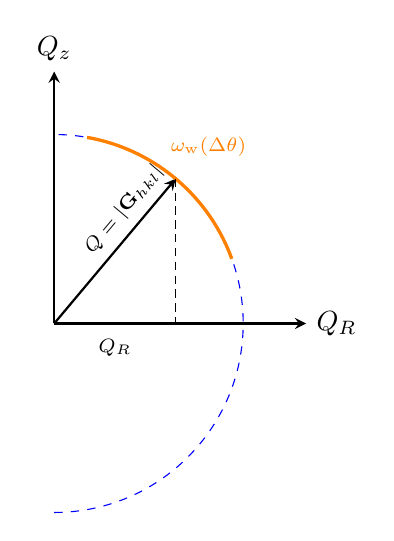
\begin{tikzpicture}[scale=2,>=stealth]
  \def\R{1.2}        % Bragg-sphere radius
  \def\Raxis{1.6}    % axis length
  \def\angleMid{50}  % midpoint angle of mosaic arc (degrees)

  % Folded Bragg locus in the radial coordinate Q_R >= 0
  \draw[dashed,blue] (0,-\R) arc (-90:90:\R);

  % reciprocal-space axes
  \draw[->,thick] (0,0) -- (0,\Raxis) node[above] {$Q_z$};
  \draw[->,thick] (0,0) -- (\Raxis,0) node[right] {$Q_R$};

  % radius vector at midpoint of mosaic arc, label closer to tip
  \coordinate (Gvec) at ({\R*cos(\angleMid)},{\R*sin(\angleMid)});
  \draw[thick,->] (0,0) -- (Gvec)
       node[pos=0.7, above, sloped] {\scriptsize $Q=|\mathbf G_{hkl}|$};

  % mosaic arc on the Bragg sphere, labeled with omega(theta)
  \draw[very thick,orange]
    ({\R*cos(20)},{\R*sin(20)}) arc (20:80:\R)
    node[pos=0.6, above right] {\scriptsize $\omega_{\mathrm w}(\Delta\theta)$};

  % projection onto the radial reciprocal-space axis
  \coordinate (Gr) at ({\R*cos(\angleMid)},0);
  \draw[densely dashed] (Gvec) -- (Gr);
  \node[below, yshift = -2pt] at ({0.5*\R*cos(\angleMid)},0) {\scriptsize $Q_R$};

\end{tikzpicture}
}
    \phantomcaption
    \label{fig:mosaic_combo:schem_inplane}
  \end{subfigure}\hfill
  \begin{subfigure}[t]{0.48\linewidth}
    \centering
    \paneltagged{(b)}{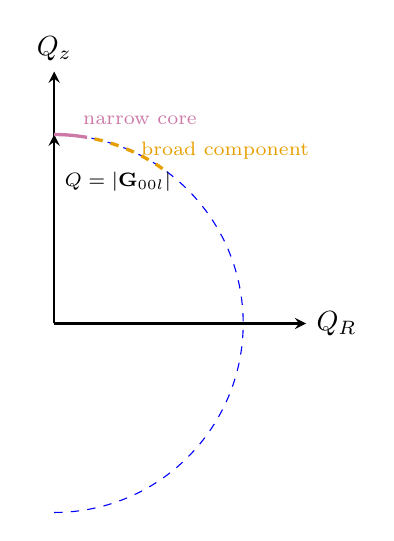
\begin{tikzpicture}[scale=2,>=stealth]
  \def\R{1.2}
  \def\Raxis{1.6}
  \def\angleMid{90}

  % Folded Bragg locus in the radial coordinate Q_R >= 0
  \draw[dashed,blue] (0,-\R) arc (-90:90:\R);

  % Reciprocal-space axes
  \draw[->,thick] (0,0) -- (0,\Raxis) node[above] {$Q_z$};
  \draw[->,thick] (0,0) -- (\Raxis,0) node[right] {$Q_R$};

  % Specular reciprocal vector
  \coordinate (Gvec) at ({\R*cos(\angleMid)},{\R*sin(\angleMid)});
  \draw[thick,->] (0,0) -- (Gvec)
       node[pos=0.75, right] {\scriptsize $Q=|\mathbf G_{00l}|$};

  % Narrow core near the axis and broad component at larger tilt
  \draw[very thick,oiPurple]
    ({\R*cos(80)},{\R*sin(80)}) arc (80:90:\R)
    node[pos=0.45, above right, text=oiPurple] {\scriptsize narrow core};
  \draw[very thick,oiOrange,dashed]
    ({\R*cos(55)},{\R*sin(55)}) arc (55:80:\R)
    node[pos=0.45, right, text=oiOrange] {\scriptsize broad component};
\end{tikzpicture}
}
    \phantomcaption
    \label{fig:mosaic_combo:schem_specular}
  \end{subfigure}

  \vspace{0.6em}

  \begin{subfigure}[t]{0.48\linewidth}
    \centering
    \paneltagged{(c)}{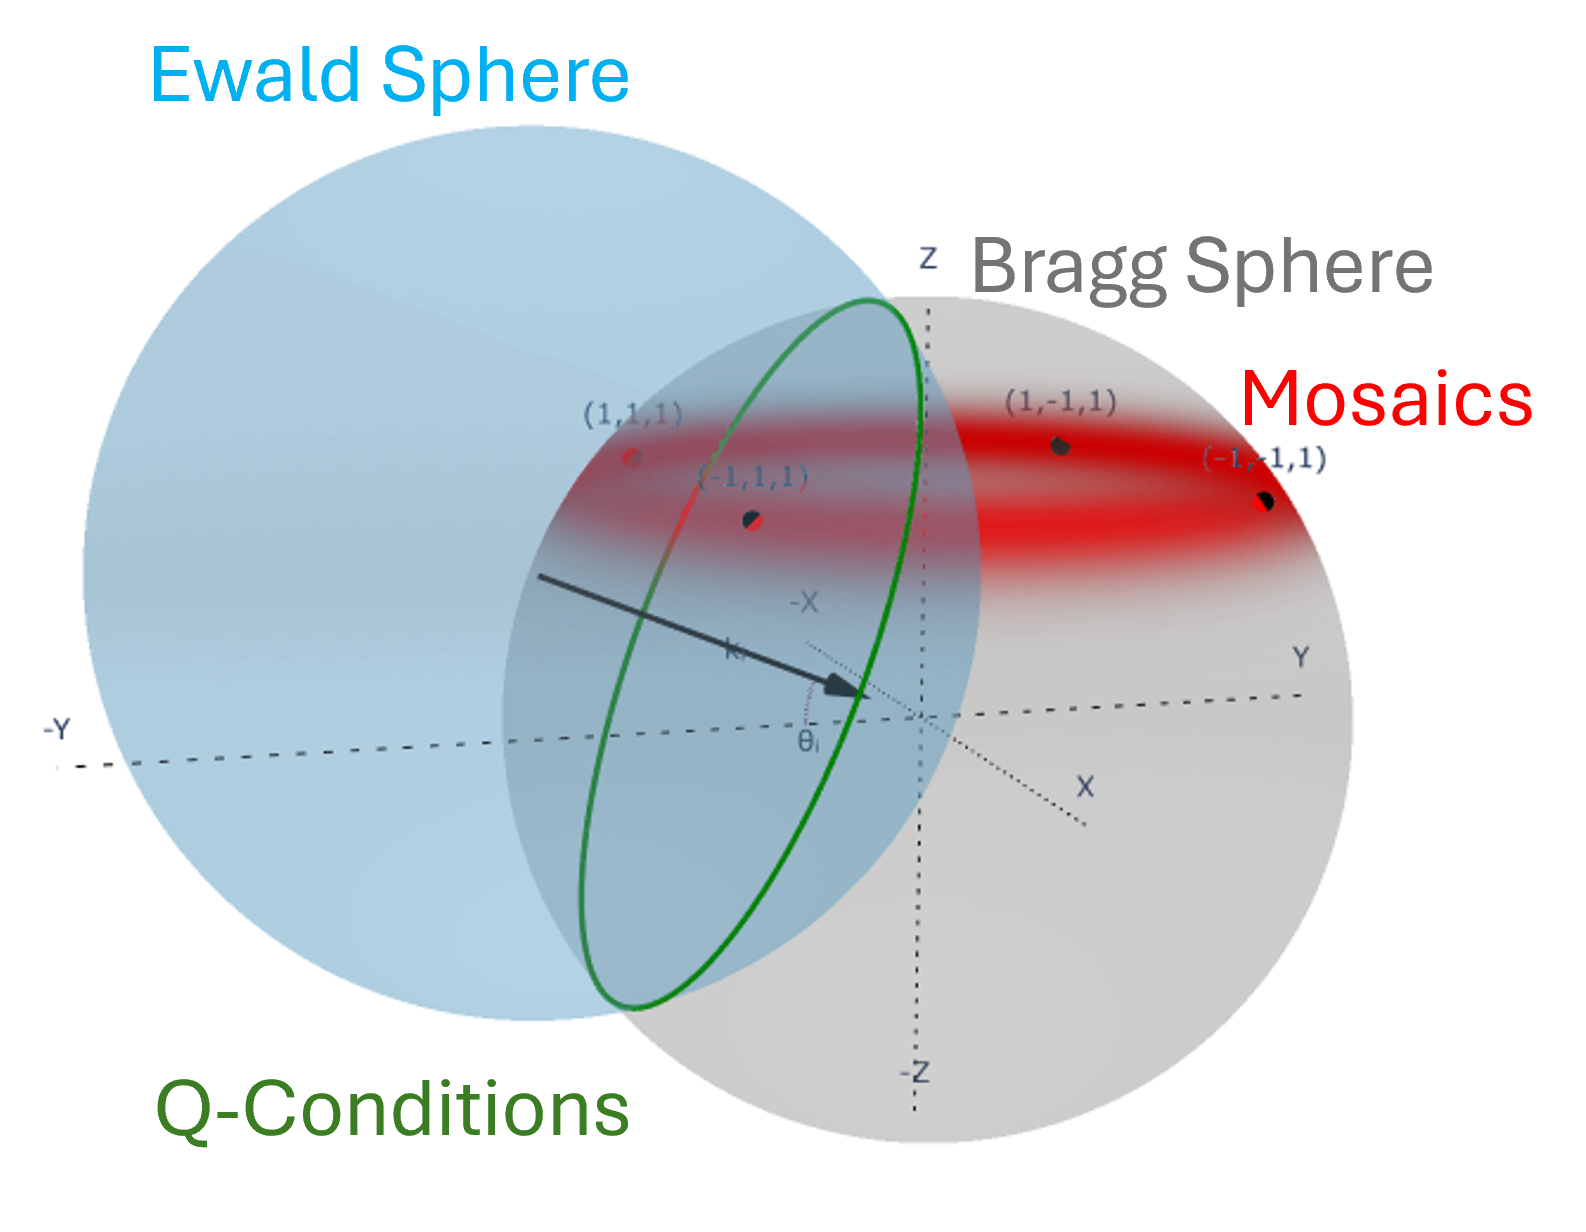
\includegraphics[width=\linewidth]{figures/mosaic/inplane_detector_band.png}}
    \phantomcaption
    \label{fig:mosaic_combo:img_inplane}
  \end{subfigure}\hfill
  \begin{subfigure}[t]{0.48\linewidth}
    \centering
    \paneltagged{(d)}{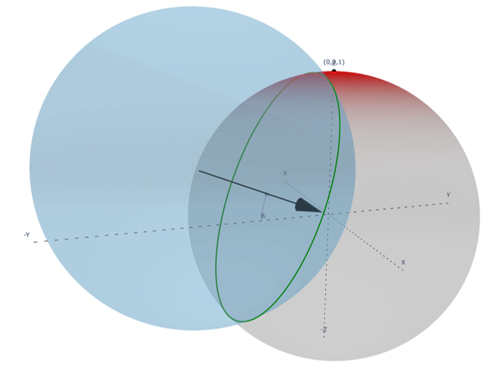
\includegraphics[width=\linewidth]{figures/mosaic/specular_detector_cap.png}}
    \phantomcaption
    \label{fig:mosaic_combo:img_specular}
  \end{subfigure}

  \caption{Geometric sensitivity to the narrow and broad crystallite-tilt components. (a) For $r\neq0$, the reciprocal vector has radial and film-normal components $Q_R$ and $Q_z$. The purple segment identifies the narrow core that predominantly controls the strong off-specular arc width, while the dashed orange extension identifies the broad, low-probability component. (b) For $r=0$, the same orientation distribution begins on the film-normal axis. Intensity displaced in the transverse $\phi$ direction samples larger crystallite tilts and is therefore more sensitive to the broad component. This transverse mosaic effect is distinct from the radial $2\theta$ streak through $003$, which is assigned primarily to wavelength dispersion in Fig.~\ref{fig:hk0_low_l_star}. Opposite tilts fold onto the same $Q_R\ge0$ locus. (c,d) Three-dimensional views place the corresponding orientation distributions relative to the Ewald-sphere intersection. The schematic illustrates sensitivity and does not replace a controlled mosaic-component comparison.}
  \label{fig:mosaic_combo}
\end{figure}

\section{Refinement workflow}
\label{sec:refinement_workflow}

Several parameter groups affect the same detector features. Detector distance changes their positions, sample alignment changes the incident condition, and mosaicity and source spread can both change widths. Refinement is staged to reduce compensation between parameter groups. Beam and detector quantities are established first, followed by sample alignment and orientation. Intensity differences are interpreted structurally after these geometric and angular constraints are established.

Table~\ref{tab:refinement_workflow} identifies the data and observables used at each stage. Instrumental parameters can be shared by measurements made in the same configuration. Sample-dependent parameters describe the film orientation, structural intensity, and, for PbI$_2$, stacking correlations.

\begin{table}[!ht]
  \centering
  \caption{Staged refinement workflow. Steps 1--5 describe the ordered Bi$_2$Se$_3$ and Bi$_2$Te$_3$ test cases. Step 6 is the added PbI$_2$ extension for stacking-fault diffuse scattering. All sample images are dark-subtracted before the listed observables are formed. A quantitative comparison requires measured and directly calculated profiles to use the same calibrated coordinate map, finite integration limits, and normalization.}
  \label{tab:refinement_workflow}
  \scriptsize
  \setlength{\tabcolsep}{3pt}
  \renewcommand{\arraystretch}{1.08}
  \begin{tabularx}{\linewidth}{@{}c >{\raggedright\arraybackslash}p{2.45cm} >{\raggedright\arraybackslash}X >{\raggedright\arraybackslash}X >{\raggedright\arraybackslash}p{2.75cm}@{}}
    \toprule
    Step & Stage & Data & Parameters refined & Primary information \\
    \midrule
    1 &
    Beam characterization &
    Direct-beam images at several detector distances &
    Beam widths $w_x$, $w_z$ and divergences $\Delta\theta_x$, $\Delta\theta_z$ &
    Incident phase space \\
    2 &
    Detector geometry calibration &
    Powder calibrant image &
    Detector distance $D$, detector tilts $(\beta_D,\gamma_D)$, and beam center $(x_0,y_0)$ &
    Detector mapping \\
    3 &
    Sample alignment and goniometer misalignment &
    Indexed reflection centers from sample images &
    Sample geometry $(\theta_i,z_B,z_S)$, in-plane rotation $\chi$, goniometer misalignment $(\alpha,\psi)$ &
    Detector-space peak positions \\
    4 &
    Mosaicity/profile refinement &
    Selected off-specular ROIs, transverse $\phi_f$ profiles, and off-condition $r=0$ regions &
    Narrow-core plus broad-component mosaic parameters &
    Off-specular arc widths, transverse $\phi_f$ widths, and off-condition axial intensity \\
    5 &
    Ordered-film comparison &
    Selected detector-space Bragg regions and $Q_z$ projections from fixed-$r$ trajectories &
    Image-wise nuisance scales and constrained ordered-intensity parameters &
    Selected Bragg-feature locations and apparent line shapes \\
    6 &
    PbI$_2$ diffuse extension &
    Fixed-$Q_R$ diffuse regions, ordered-baseline residuals, and projected $Q_z$ profiles &
    Stacking-fault probabilities or layer-pair correlation parameters &
    Diffuse intensity along $Q_z$ and separation of ordered and disorder-derived scattering \\
    \bottomrule
  \end{tabularx}
\end{table}

Direct-beam measurements constrain the beam distributions, and a powder calibrant establishes the detector mapping. Indexed sample reflections then constrain the sample pose. This geometric stage is related to detector-space indexing: it establishes where the scattering should appear before profile widths are interpreted.\cite{SmilgiesLi2026IndexGIXS}

With geometry established, off-specular and transverse axial profiles constrain the orientation distribution. Radial axial intensity depends on finite-stack scattering, orientation selection, the source distribution, and the optical response. In the model controls described in Supporting Information Sec.~S3, the radial extension persists when the source is reduced to a single monochromatic incident ray. This result does not support assigning that extension to wavelength dispersion alone.

A quantitative test of the ordered-film model requires directly calculated profiles integrated over the same finite regions as the measurements (Supporting Information Secs.~S4 and S6). For PbI$_2$, stacking variables are introduced after establishing each specimen's geometry and orientation. The added variables describe layer correlations and their effect on intensity along the rods. Source sampling is defined in Sec.~S1, finite integration in Sec.~S4, and refinement objectives, numerical convergence, and uncertainty propagation in Sec.~S8 of the Supporting Information.

\section{Validation: Bi\texorpdfstring{$_2$}{2}Se\texorpdfstring{$_3$}{3} and Bi\texorpdfstring{$_2$}{2}Te\texorpdfstring{$_3$}{3} films}
\label{sec:results_ordered}

Ordered Bi$_2$Se$_3$ and Bi$_2$Te$_3$ films provide validation. Detector images collected at incident angles of $5^\circ$, $10^\circ$, and $15^\circ$ entered the staged refinement. Figures~\ref{fig:ordered_bi2se3_test} and~\ref{fig:ordered_bi2te3_test} show the $5^\circ$ condition because it displays both the selected off-specular rod families and the $r=0$ features clearly within one detector image while the others can be found in the supplemental materials.

$r\neq0$ rods are naturally described by $Q$ space and integrated along $Q_R$ as a function of $L$. Mosaic and beam sampling distort the projection to $\mathbf Q$ and thus the plotted curves therefore compare the same detector-derived observable rather than an ideal reciprocal-space line cut. Meanwhile, $r=0$ rods are described best integrated along $\phi$ as a function of $2\theta$.

In the detector panels, solid colored curves mark calculated trajectory centerlines. Semi-transparent bands show the regions integrated for the profiles, and dashed outlines mark their boundaries. The central blue region follows the $r=0$ family. Paired off-specular regions are the two detector-side intersections of one $r$ family, identified by plus and minus signs. In the profile panels, black solid curves are measured data and orange dashed curves are the corresponding calculations. The horizontal coordinate is $L$, with integer markers denoting nominal Bragg conditions along the selected trajectory. Off-specular rows are plotted on a linear scale, while the $r=0$ row is plotted logarithmically to display weak off-condition intensity. Along the $r=0$ trajectory, the radial $L$ or $2\theta$ line shape contains the wavelength convolution, whereas the transverse $\phi$ width provides the cleaner mosaic constraint.

\begin{figure}[p]
  \centering
  \captionsetup{font=footnotesize}
  {\large\bfseries Measured detector image and selected trajectory bands\par}
  \vspace{0.35em}
  \begin{minipage}{0.78\linewidth}
    \centering
    \draftfigureplaceholder[0.28\textheight]{figures/results_ordered/figure7_bi2se3_qr_rod_qz_profiles_detector_selected_q_regions_5deg.png}{%
      Bi$_2$Se$_3$ detector image with selected fixed-$Q_R$ trajectory centerlines and finite profile-integration regions.
    }
  \end{minipage}

  \vspace{0.35em}
  {\large\bfseries Matched projected profiles\par}
  \vspace{0.25em}
  \begin{minipage}{0.56\linewidth}
    \centering
    \draftfigureplaceholder[0.35\textheight]{figures/results_ordered/figure7_bi2se3_qr_rod_qz_profiles.png}{%
      Bi$_2$Se$_3$ measured and calculated profiles for the selected detector regions.
    }
  \end{minipage}
  \caption[Bi2Se3 detector-space test case]{Bi$_2$Se$_3$ detector-space comparison at $\theta_i=5^\circ$. The upper panel is the measured detector image with calculated trajectory centerlines, finite integration regions, and their boundaries. Labels $r$ identify radial rod families, while plus and minus signs distinguish the two detector-side intersections of one off-specular family. The lower panel compares measured black curves with calculated orange dashed curves generated using the same coordinate map, integration limits, and area normalization. The figure tests trajectory placement and apparent profile line shape. In the $r=0$ family, radial broadening is evaluated with the wavelength distribution, while the transverse $\phi$ width is used to constrain mosaicity. Separate family amplitudes are not a common-scale relative-intensity test, and the $r=0$ row does not establish a unique broad-component functional form.}
  \label{fig:ordered_bi2se3_test}
\end{figure}

\begin{figure}[p]
  \centering
  \captionsetup{font=footnotesize}
  {\large\bfseries Measured detector image and selected trajectory bands\par}
  \vspace{0.35em}
  \begin{minipage}{0.78\linewidth}
    \centering
    \draftfigureplaceholder[0.28\textheight]{figures/results_ordered/figure7_bi2te3_qr_rod_qz_profiles_detector_selected_q_regions_5deg.png}{%
      Bi$_2$Te$_3$ detector image with selected fixed-$Q_R$ trajectory centerlines and finite profile-integration regions.
    }
  \end{minipage}

  \vspace{0.35em}
  {\large\bfseries Matched projected profiles\par}
  \vspace{0.25em}
  \begin{minipage}{0.56\linewidth}
    \centering
    \draftfigureplaceholder[0.35\textheight]{figures/results_ordered/figure7_bi2te3_qr_rod_qz_profiles.png}{%
      Bi$_2$Te$_3$ measured and calculated profiles for the selected detector regions.
    }
  \end{minipage}
  \caption[Bi2Te3 detector-space test case]{Bi$_2$Te$_3$ detector-space comparison at $\theta_i=5^\circ$, using the conventions of Fig.~\ref{fig:ordered_bi2se3_test}. The upper panel shows the measured detector image with calculated trajectories and finite integration regions. The lower panel compares detector-derived profiles formed with the same coordinate transformation, finite integration, and area normalization. The principal peaks occur at the same projected locations and have similar apparent line shapes within the displayed fitted condition. Separate family amplitudes are not interpreted on one common physical scale, and the $r=0$ profile is not proof of a unique broad mosaic component.}
  \label{fig:ordered_bi2te3_test}
\end{figure}

Mosaicity, beam divergence, wavelength spread, incidence-angle uncertainty, calibrated detector mapping, and finite integration width all broaden the effective scattering condition. The projected coordinate should therefore not be interpreted as an exact cut through the reciprocal space of one perfect crystallite. The comparison remains direct because the same coordinate transformation and finite integration operation are applied to the calculated and measured detector quantities.

The off-specular and $r=0$ features play complementary roles. The off-specular arcs test the two-dimensional-powder reciprocal-space construction and calibrated detector geometry. Their transverse widths and asymmetries constrain the effective narrow mosaic component together with beam divergence and finite integration width. For the $r=0$ family, the radial $2\theta$ or $L$ shape is sensitive to the wavelength distribution and the specular intensity envelope, while the transverse $\phi$ width is the cleaner probe of the broad orientation component. The full-spectrum versus mean-wavelength comparison in Sec.~\ref{sec:correlated_effects} isolates the radial $003$ streak from the mosaic-sensitive transverse width. The displayed overlays show that the fitted model can represent the selected feature locations and apparent profile shapes. A controlled Gaussian-only comparison is still required before the broad component can be called necessary or uniquely Lorentzian.


\section{Results: diffuse scattering and stacking disorder in PbI\texorpdfstring{$_2$}{2}}
\label{sec:results_pbi2}

Figure~\ref{fig:pbi2_diffuse_cylinders} shows a CVD-grown PbI$_2$ film and a crop spanning the $r=0$ and $r=1$ reciprocal rods. The $r=1$ rod contains measurable intensity between the integer Bragg maxima, whereas the $r=0$ rod is dominated by sharp peaks and finite-thickness oscillations. This rod-dependent redistribution is the experimental motivation for the stacking-disorder model. In a two-dimensional powder, random in-plane orientation maps each $(h,k)$ rod onto a reciprocal-space cylinder at fixed $Q_R$. An infinite ordered crystal gives intensity at discrete crystallite-frame $L$ values, while a finite ordered stack already produces a continuous $S_{hk}(L)$ with finite widths and fringes. Stacking faults do not create these rods. They change the correlations among trilayers and redistribute intensity within the existing continuous rod profile.

\begin{figure}[H]
  \centering
  \begin{minipage}{0.78\linewidth}
    \centering
    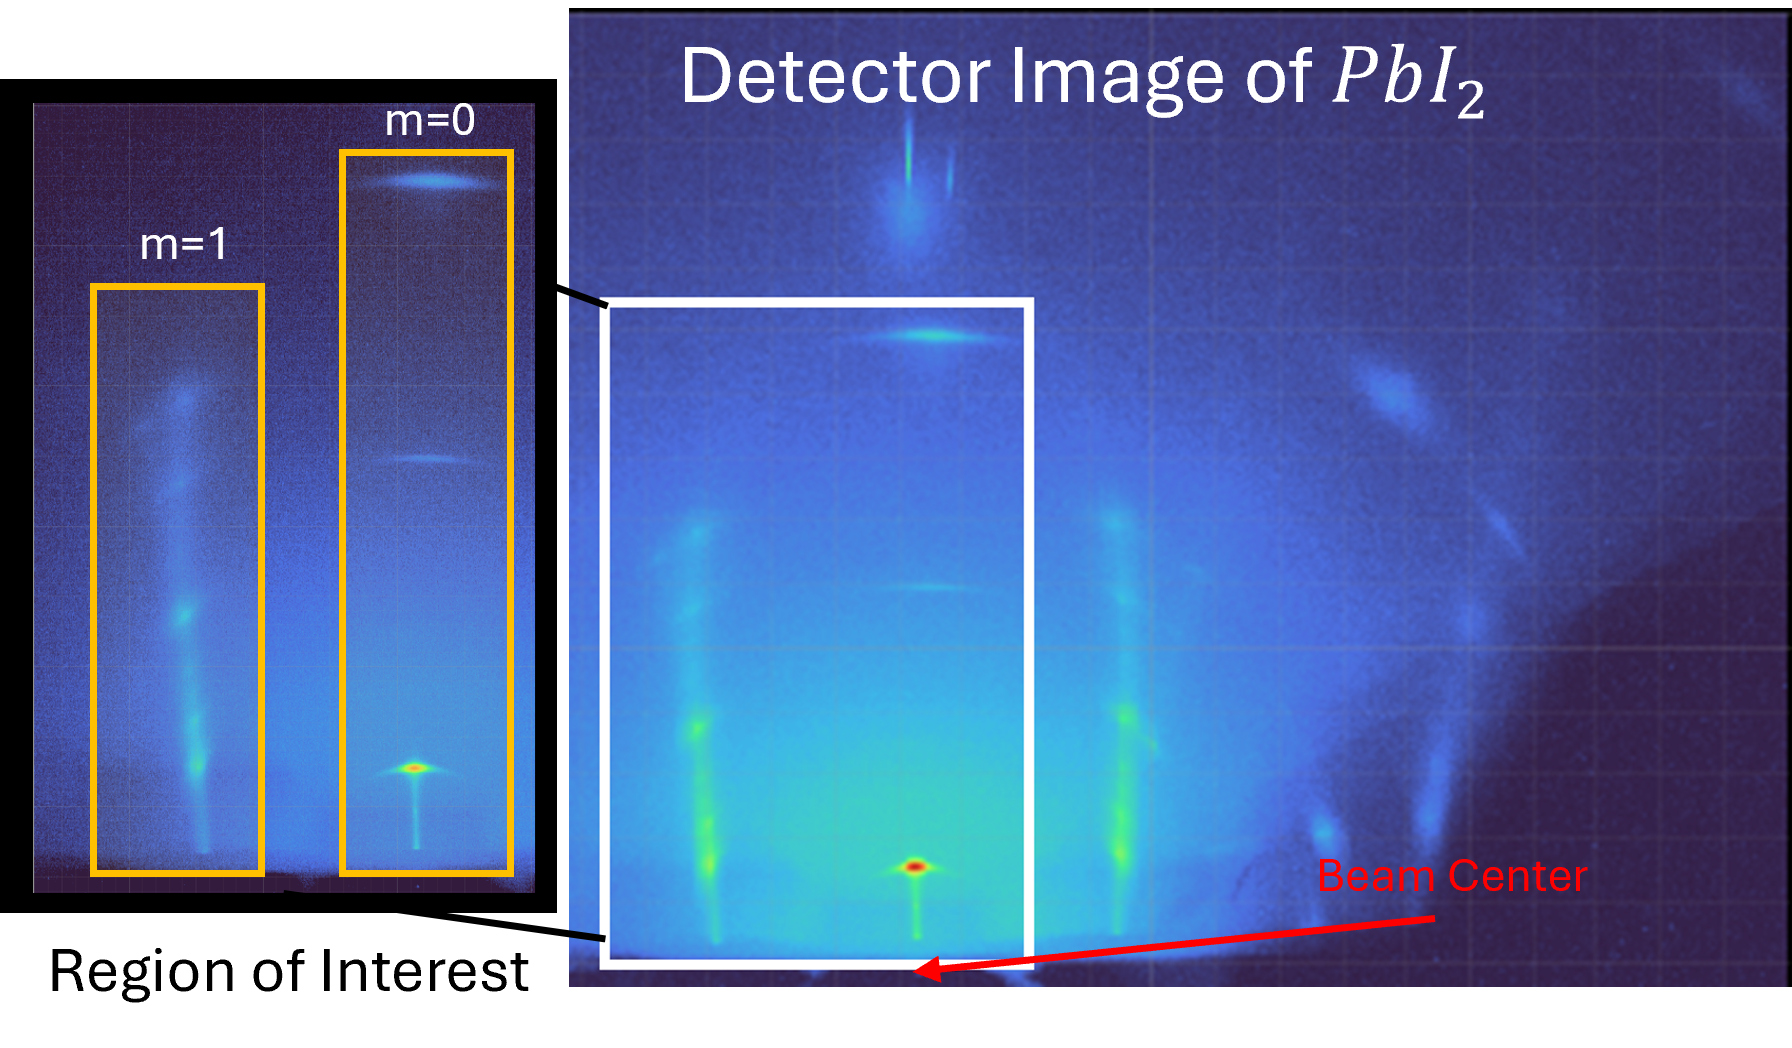
\includegraphics[width=\linewidth]{figures/results_pbi2/PbI2_detector.png}
  \end{minipage}
  \caption{Measured PbI$_2$ diffraction image (right) and an enlarged region of interest (left). The direct-beam position defines the vertical $r=0$ trajectory. Diffuse intensity is visible between the ordered maxima on the neighboring $r=1$ rod, while the $r=0$ profile is contrast-matched to the basal-plane shifts included in the stacking model.}
  \label{fig:pbi2_diffuse_cylinders}
\end{figure}

The contrast between the two rods identifies the structural information carried by the diffuse intensity. A forward basal-plane shift $\mathbf s=(1/3,2/3)$ multiplies the amplitude of one $(h,k)$ rod by
\begin{equation}
  \omega_{hk}=\exp\!\left[2\pi i(hs_x+ks_y)\right]
  =\exp\!\left[\frac{2\pi i}{3}(h+2k)\right].
  \label{eq:pbi2_registry_phase}
\end{equation}
For $h=k=0$, $\omega_{00}=1$, and the two trilayer orientations have the same $00L$ amplitude in the present model. The $r=0$ rod is therefore insensitive to the included basal-plane shifts and orientation changes: faults can be present, but they are contrast-matched on that rod. Off-specular rods retain the lateral phase contrast, so the same faults change their pair interference and transfer intensity from ordered maxima into the diffuse regions between them.

\subsection{From stacking faults to rod intensity}
\label{sec:pbi2_transition_model}

The structural unit is one I--Pb--I trilayer. Its state is described by a basal-plane position $\rho\in\{0,1,2\}$ and an orientation $\sigma\in\{+,-\}$. The ordered 2H, 4H, and 6H parents are deterministic sequences of these six possible layer states. Figure~\ref{fig:pbi2_transition_states} renders the corresponding cycles as projected I--Pb--I stacks. Read from bottom to top, they are $0F_+\rightarrow0F_+$ for 2H, $0F_+\rightarrow1F_-\rightarrow0F_+$ for 4H, and $0F_+\rightarrow1F_+\rightarrow2F_+\rightarrow0F_+$ for 6H. The existence and crystallographic stacking sequences of these parent polytypes are established experimentally.\cite{Minagawa1975,Palosz1990}

\begin{figure}[H]
  \centering
  \resizebox{0.88\linewidth}{!}{%
    % PbI2 polytype-stack schematic rendered directly by main.tex.
% Required packages/libraries are loaded in the manuscript preamble:
% tikz, xcolor, and the calc and arrows.meta TikZ libraries.
\begingroup

\definecolor{iodine}{RGB}{145,20,145}
\definecolor{lead}{RGB}{74,76,82}
\definecolor{guideblue}{RGB}{0,105,145}
\definecolor{guidegreen}{RGB}{55,175,35}
\definecolor{chargecyan}{RGB}{0,205,225}

\tikzset{
	cell edge/.style={
		draw=black!70,
		line width=0.45pt
	},
	blue guide/.style={
		draw=guideblue,
		line width=0.65pt,
		dash pattern=on 2.3pt off 2.0pt
	},
	green guide/.style={
		draw=guidegreen,
		line width=0.65pt,
		dash pattern=on 2.3pt off 2.0pt
	},
	bracket/.style={
		draw=black,
		line width=0.75pt,
		line cap=round,
		line join=round
	},
	panel title/.style={
		font=\sffamily\bfseries\fontsize{13}{14}\selectfont,
		text=black!85
	},
	stack label/.style={
		font=\sffamily\bfseries\fontsize{14}{15}\selectfont,
		text=black!80
	}
}

% Pb--I bond: dark outer cylinder, gray Pb half, violet I half.
\newcommand{\PbIbond}[2]{%
	\draw[
	black!72,
	line width=1.55pt,
	line cap=round
	] (#1) -- (#2);
	
	\draw[
	lead!92,
	line width=0.86pt,
	line cap=round
	] (#1) -- ($(#1)!0.53!(#2)$);
	
	\draw[
	iodine!95,
	line width=0.86pt,
	line cap=round
	] ($(#1)!0.47!(#2)$) -- (#2);
}

\newcommand{\Iatom}[1]{%
	\shade[ball color=iodine]
	(#1) circle[radius=13];
	
	\draw[
	black!55,
	line width=0.22pt
	] (#1) circle[radius=13];
}

\newcommand{\Pbatom}[1]{%
	\shade[ball color=lead]
	(#1) circle[radius=18];
	
	\draw[
	black!60,
	line width=0.25pt
	] (#1) circle[radius=18];
}

% Coordinates for an A layer.
% #1 = coordinate prefix.
% #2 = y coordinate of the upper iodine row.
\newcommand{\NormalAcoords}[2]{%
	\coordinate (#1T1) at (174,{#2});
	\coordinate (#1T2) at (273,{#2});
	\coordinate (#1T3) at (372,{#2});
	
	\coordinate (#1P1) at (239,{#2+47});
	\coordinate (#1P2) at (338,{#2+47});
	
	\coordinate (#1B1) at (207,{#2+93});
	\coordinate (#1B2) at (305,{#2+93});
	\coordinate (#1B3) at (404,{#2+93});
}

% Coordinates for a B layer.
\newcommand{\Bcoords}[2]{%
	\coordinate (#1T1) at (207,{#2});
	\coordinate (#1T2) at (305,{#2});
	
	\coordinate (#1P) at (273,{#2+47});
	
	\coordinate (#1B1) at (239,{#2+93});
	\coordinate (#1B2) at (338,{#2+93});
}

% B layer flipped about its fixed Pb position.
\newcommand{\Binvcoords}[2]{%
	\coordinate (#1T1) at (239,{#2});
	\coordinate (#1T2) at (338,{#2});
	
	\coordinate (#1P) at (273,{#2+47});
	
	\coordinate (#1B1) at (207,{#2+93});
	\coordinate (#1B2) at (305,{#2+93});
}

\newcommand{\DrawNormalA}[1]{%
	\PbIbond{#1P1}{#1T1}
	\PbIbond{#1P1}{#1T2}
	\PbIbond{#1P1}{#1B1}
	\PbIbond{#1P1}{#1B2}
	
	\PbIbond{#1P2}{#1T2}
	\PbIbond{#1P2}{#1T3}
	\PbIbond{#1P2}{#1B2}
	\PbIbond{#1P2}{#1B3}
	
	\Iatom{#1T1}
	\Iatom{#1T2}
	\Iatom{#1T3}
	
	\Iatom{#1B1}
	\Iatom{#1B2}
	\Iatom{#1B3}
	
	\Pbatom{#1P1}
	\Pbatom{#1P2}
}

\newcommand{\DrawB}[1]{%
	\PbIbond{#1P}{#1T1}
	\PbIbond{#1P}{#1T2}
	\PbIbond{#1P}{#1B1}
	\PbIbond{#1P}{#1B2}
	
	\Iatom{#1T1}
	\Iatom{#1T2}
	
	\Iatom{#1B1}
	\Iatom{#1B2}
	
	\Pbatom{#1P}
}

\newcommand{\DrawBinv}[1]{%
	\PbIbond{#1P}{#1T1}
	\PbIbond{#1P}{#1T2}
	\PbIbond{#1P}{#1B1}
	\PbIbond{#1P}{#1B2}
	
	\Iatom{#1T1}
	\Iatom{#1T2}
	
	\Iatom{#1B1}
	\Iatom{#1B2}
	
	\Pbatom{#1P}
}

	\begin{tikzpicture}[x=0.1mm,y=-0.1mm]
		
		% Compact two-column layout:
		% 2H above 4H on the left.
		% 2H monolayer above 6H on the right.
		\path[use as bounding box]
		(0,0) rectangle (900,990);
		
		% ================================================================
		% Top left: 2H
		% ================================================================
		\begin{scope}[shift={(-40,0)}]
			
			\node[panel title] at (289,18) {(a) 2H};
			
			\NormalAcoords{hU}{60}
			\NormalAcoords{hL}{225}
			
			% Projected unit-cell edges.
			\draw[cell edge]
			(hUP1) -- (hUP2);
			
			\draw[cell edge]
			(hUP1) -- (hLP1);
			
			\draw[cell edge]
			(hUP2) -- (hLP2);
			
			\draw[cell edge]
			(hLP1) -- (hLP2);
			
			\DrawNormalA{hU}
			\DrawNormalA{hL}
			
			% Registry guides.
			\draw[green guide]
			(239,60) -- (239,355);
			
			\draw[green guide]
			(272,60) -- (272,355);
			
			\draw[green guide]
			(306,60) -- (306,355);
			
			\draw[green guide]
			(338,60) -- (338,355);
			
			\draw[blue guide]
			(174,225) -- (405,225);
			
			\draw[blue guide]
			(239,272) -- (386,272);
			
			\draw[blue guide]
			(207,318) -- (418,318);
			
			% Restore the rightmost lower iodine above the dashed guide.
			\Iatom{hLB3}
			
			% Ionic signs on the reference A layer.
			\foreach \a in {hLT1,hLT2,hLT3,hLB1,hLB2,hLB3}{
				\node[
				text=chargecyan,
				font=\bfseries\fontsize{9}{9}\selectfont
				] at (\a) {$-$};
			}
			
			\foreach \a in {hLP1,hLP2}{
				\node[
				text=guidegreen!85!black,
				font=\bfseries\fontsize{9}{9}\selectfont
				] at (\a) {$+$};
			}
			
			% Layer brackets.
			\draw[bracket]
			(150,60)
			-- (134,60)
			-- (134,153)
			-- (150,153);
			
			\draw[bracket]
			(150,225)
			-- (134,225)
			-- (134,318)
			-- (150,318);
			
			% Stacking labels.
			\node[stack label] at (98,107)
			{$0F_{+}$};
			
			\node[stack label] at (98,272)
			{$0F_{+}$};
			
		\end{scope}
		
		% ================================================================
		% Bottom left: 4H
		% ================================================================
		\begin{scope}[shift={(-40,385)}]
			
			\node[panel title] at (289,18) {(c) 4H};
			
			\Binvcoords{fU}{60}
			\NormalAcoords{fL}{225}
			
			% Projected unit-cell edges.
			\draw[cell edge]
			(239,107) -- (338,107);
			
			\draw[cell edge]
			(239,107) -- (fLP1);
			
			\draw[cell edge]
			(338,107) -- (fLP2);
			
			\draw[cell edge]
			(fLP1) -- (fLP2);
			
			\DrawBinv{fU}
			\DrawNormalA{fL}
			
			% Registry guides.
			\draw[green guide]
			(239,60) -- (239,355);
			
			\draw[green guide]
			(272,60) -- (272,355);
			
			\draw[green guide]
			(306,60) -- (306,355);
			
			\draw[green guide]
			(338,60) -- (338,355);
			
			\draw[blue guide]
			(174,225) -- (405,225);
			
			\draw[blue guide]
			(239,272) -- (386,272);
			
			\draw[blue guide]
			(207,318) -- (418,318);
			
			% Restore the rightmost lower iodine above the dashed guide.
			\Iatom{fLB3}
			
			% Ionic signs on the reference A layer.
			\foreach \a in {fLT1,fLT2,fLT3,fLB1,fLB2,fLB3}{
				\node[
				text=chargecyan,
				font=\bfseries\fontsize{9}{9}\selectfont
				] at (\a) {$-$};
			}
			
			\foreach \a in {fLP1,fLP2}{
				\node[
				text=guidegreen!85!black,
				font=\bfseries\fontsize{9}{9}\selectfont
				] at (\a) {$+$};
			}
			
			% Layer brackets.
			\draw[bracket]
			(150,60)
			-- (134,60)
			-- (134,153)
			-- (150,153);
			
			\draw[bracket]
			(150,225)
			-- (134,225)
			-- (134,318)
			-- (150,318);
			
			% Stacking labels.
			\node[stack label] at (93,107)
			{$1F_{-}$};
			
			\node[stack label] at (98,272)
			{$0F_{+}$};
			
		\end{scope}
		
		% ================================================================
		% Top right: single A layer of 2H
		% ================================================================
		\begin{scope}[shift={(420,0)}]
			
			\node[panel title] at (289,18)
			{(b) $F_{+}$ trilayer};
			
			\NormalAcoords{m}{65}
			
			% Projected in-plane cell edge.
			\draw[cell edge]
			(mP1) -- (mP2);
			
			\DrawNormalA{m}
			
			% Reference guides and labels appear only in this panel.
			\draw[green guide]
			(239,65) -- (239,205);
			
			\draw[green guide]
			(272,65) -- (272,205);
			
			\draw[green guide]
			(306,65) -- (306,205);
			
			\draw[green guide]
			(338,65) -- (338,205);
			
			\draw[blue guide]
			(174,65) -- (405,65);
			
			\draw[blue guide]
			(239,112) -- (386,112);
			
			\draw[blue guide]
			(207,158) -- (418,158);
			
			% Restore the rightmost lower iodine above the dashed guide.
			\Iatom{mB3}
			
			% Ionic signs.
			\foreach \a in {mT1,mT2,mT3,mB1,mB2,mB3}{
				\node[
				text=chargecyan,
				font=\bfseries\fontsize{9}{9}\selectfont
				] at (\a) {$-$};
			}
			
			\foreach \a in {mP1,mP2}{
				\node[
				text=guidegreen!85!black,
				font=\bfseries\fontsize{9}{9}\selectfont
				] at (\a) {$+$};
			}
			
			% Atomic-plane labels.
			\node[
			anchor=west,
			font=\fontsize{11}{12}\selectfont
			] at (400,65) {$\mathrm{I}_{2}$};
			
			\node[
			anchor=west,
			font=\fontsize{11}{12}\selectfont
			] at (379,114) {$\mathrm{Pb}$};
			
			\node[
			anchor=west,
			font=\fontsize{11}{12}\selectfont
			] at (425,160) {$\mathrm{I}_{1}$};
			
			% In-plane phase axis aligned with the green registry guides.
			\draw[black!70,line width=0.45pt]
			(239,210) -- (338,210);
			
			\foreach \x/\lab in {239/{$0$},272/{$\displaystyle\frac{\pi}{3}$},306/{$\displaystyle\frac{2\pi}{3}$},338/{$\pi$}}{
				\draw[black!70,line width=0.45pt] (\x,207) -- (\x,213);
				\node[
				font=\fontsize{6.5}{7}\selectfont,
				anchor=north east,
				rotate=65
				] at (\x,216) {\lab};
			}
			
			\node[
			font=\fontsize{7}{8}\selectfont,
			anchor=west
			] at (347,210) {registry phase};

		\end{scope}
		
		% ================================================================
		% Bottom right: 6H
		% ================================================================
		\begin{scope}[shift={(420,335)}]
			
			\node[panel title] at (289,18) {(d) 6H};
			
			\NormalAcoords{sU}{50}
			\NormalAcoords{sL}{500}
			
			% C layer.
			\coordinate (sCT1) at (239,200);
			\coordinate (sCT2) at (339,200);
			
			\coordinate (sCP) at (305,247);
			
			\coordinate (sCB1) at (273,293);
			\coordinate (sCB2) at (371,293);
			
			% B layer.
			\Bcoords{sM}{350}
			
			% Projected unit-cell edges.
			\draw[cell edge]
			(sUP1) -- (sUP2);
			
			\draw[cell edge]
			(sUP1) -- (sLP1);
			
			\draw[cell edge]
			(sUP2) -- (sLP2);
			
			\draw[cell edge]
			(sLP1) -- (sLP2);
			
			% Top A layer.
			\DrawNormalA{sU}
			
			% C layer.
			\PbIbond{sCP}{sCT1}
			\PbIbond{sCP}{sCT2}
			\PbIbond{sCP}{sCB1}
			\PbIbond{sCP}{sCB2}
			
			\Iatom{sCT1}
			\Iatom{sCT2}
			\Iatom{sCB1}
			\Iatom{sCB2}
			
			\Pbatom{sCP}
			
			% B and lower A layers.
			\DrawB{sM}
			\DrawNormalA{sL}
			
			% Registry guides.
			\draw[green guide]
			(272,50) -- (272,625);
			
			\draw[green guide]
			(306,50) -- (306,625);
			
			\draw[green guide]
			(239,547) -- (239,625);
			
			\draw[green guide]
			(338,547) -- (338,625);
			
			\draw[blue guide]
			(174,500) -- (405,500);
			
			\draw[blue guide]
			(239,547) -- (386,547);
			
			\draw[blue guide]
			(207,593) -- (418,593);
			
			% Restore the rightmost lower iodine above the dashed guide.
			\Iatom{sLB3}
			
			% Ionic signs on the reference A layer.
			\foreach \a in {sLT1,sLT2,sLT3,sLB1,sLB2,sLB3}{
				\node[
				text=chargecyan,
				font=\bfseries\fontsize{9}{9}\selectfont
				] at (\a) {$-$};
			}
			
			\foreach \a in {sLP1,sLP2}{
				\node[
				text=guidegreen!85!black,
				font=\bfseries\fontsize{9}{9}\selectfont
				] at (\a) {$+$};
			}
			
			% Layer brackets.
			\draw[bracket]
			(150,50)
			-- (134,50)
			-- (134,143)
			-- (150,143);
			
			\draw[bracket]
			(158,200)
			-- (142,200)
			-- (142,293)
			-- (158,293);
			
			\draw[bracket]
			(164,350)
			-- (147,350)
			-- (147,443)
			-- (164,443);
			
			\draw[bracket]
			(150,500)
			-- (134,500)
			-- (134,593)
			-- (150,593);
			
			% Stacking labels.
			\node[stack label] at (98,97)
			{$0F_{+}$};
			
			\node[stack label] at (98,247)
			{$2F_{+}$};
			
			\node[stack label] at (98,397)
			{$1F_{+}$};
			
			\node[stack label] at (98,547)
			{$0F_{+}$};
			
		\end{scope}
		
		% ================================================================
		% One shared lattice-direction axis
		% ================================================================
		% Since y=-0.1mm, decreasing y points visually upward.
		\coordinate (Oax) at (28,965);
		
		\draw[
		-{Latex[length=2.2mm,width=1.6mm]},
		line width=0.8pt
		]
		(Oax) -- ++(0,-52)
		node[
		above,
		font=\sffamily\fontsize{10}{10}\selectfont
		] {$c$};
		
		\draw[
		-{Latex[length=2.2mm,width=1.6mm]},
		line width=0.8pt
		]
		(Oax) -- ++(52,0)
		node[
		right,
		font=\sffamily\fontsize{10}{10}\selectfont
		] {$a$};
		
	\end{tikzpicture}
	
\endgroup
%
  }
  \caption{Deterministic PbI$_2$ parent cycles used in the transition model. (a) 2H repeats $0F_+$. (b) The isolated $F_+$ trilayer defines the local orientation. (c) 4H alternates $0F_+$ and $1F_-$. (d) 6H advances $0F_+\rightarrow1F_+\rightarrow2F_+\rightarrow0F_+$. In a state label $\rho F_\sigma$, $\rho$ is the basal-plane position and $\sigma$ is the trilayer orientation.}
  \label{fig:pbi2_transition_states}
\end{figure}

Adjacent trilayers are connected by five allowed interface events. The event $a$ leaves the basal-plane position and orientation unchanged. The events $b_+$ and $b_-$ shift the next trilayer forward or backward without changing its orientation, while $d_+$ and $d_-$ combine those shifts with an orientation change. A change of orientation without a basal-plane shift is excluded. The parent events are $a$ for 2H, $d_+$ for 4H, and $b_+$ for 6H. Reversing the shift direction gives the symmetry-related handed counterparts.

A stacking fault is represented as a local departure from the selected parent event. For a parent-rich population $j\in\{2H,4H,6H\}$, the equal-alternative template is
\begin{equation}
  p_j(\text{parent event})=1-\epsilon_j,
  \qquad
  p_j(\text{each alternative})=\frac{\epsilon_j}{4}.
  \label{eq:pbi2_fault_parameterization}
\end{equation}
Thus $\epsilon_j$ is the effective per-interface probability of departing from the selected parent event under this template. It is not a universal PbI$_2$ fault density. The transition matrix propagates these events over multiple layer separations and calculates the phase-weighted pair correlation for each $(h,k)$ rod. The complete six-state construction, its exact rod-dependent reduction, and the finite-stack derivation are given in the Supporting Information.\cite{HendricksTeller1942,KakinokiKomura1954,KakinokiKomura1965,Hart2018}

The main physical quantity is the correlation between trilayers separated by $\Delta$ interfaces. Let $C_{hk}^{(j)}(\Delta;L,\lambda_s)$ be the disorder-averaged scattering correlation, averaged over all layer pairs at that separation, for population $j$. Let $N$ be the number of trilayers, $d$ their normal separation, and $q_z=2\pi L/c$ the crystallite-frame momentum-transfer component along the rod. The corresponding finite-stack rod intensity can be written as
\begin{equation}
  S_{hk}^{(j)}(L,\lambda_s)
  =S_{\mathrm{self},hk}^{(j)}(L,\lambda_s)
  +\frac{2}{N}\operatorname{Re}\sum_{\Delta=1}^{N-1}
  (N-\Delta)C_{hk}^{(j)}(\Delta;L,\lambda_s)e^{iq_zd\Delta}.
  \label{eq:pbi2_pair_correlation_intensity}
\end{equation}
The first term is the intensity scattered by the individual trilayers. The second is their interference, grouped by separation $\Delta$. An ordered parent preserves a periodic correlation over long separations and gives sharp maxima with finite-stack fringes. Fault events dephase or shorten that periodic correlation and transfer intensity into the diffuse regions between the maxima.

The 2H-, 4H-, and 6H-rich populations are treated as mutually incoherent, so their intensities are combined as
\begin{equation}
  S_{hk}(L,\lambda_s)=
  \sum_{j\in\{2H,4H,6H\}}w_jS_{hk}^{(j)}(L,\lambda_s),
  \qquad w_{2H}+w_{4H}+w_{6H}=1.
  \label{eq:pbi2_population_sum}
\end{equation}
This population-weighted $S_{hk}(L,\lambda_s)$ replaces the ordered finite-stack rod intensity introduced in Sec.~\ref{sec:structure_factor}. The subsequent powder-cylinder formation, mosaic broadening, Ewald selection, optical weighting, detector mapping, and finite-region integration are unchanged. The stacking model is therefore a structural module within the same detector-space forward calculation rather than a separate diffraction framework.

\subsection{Hierarchy of stacking-disorder models}
\label{sec:pbi2_model_hierarchy}

The selected comparisons should be organized as a nested model hierarchy rather than as a generic low-to-high disorder series. The first stage establishes a nearly ordered 2H baseline. The second asks whether faults within a 2H-rich population alone reproduce the diffuse redistribution. The third adds a 6H-rich population, and the fourth adds a 4H-rich population. Each stage must use the same detector geometry, background treatment, integration regions, and ordered baseline, and added complexity is retained only when it improves the fault-sensitive rod profiles without degrading the ordered maxima.

\begin{figure}[H]
  \centering
  {\large\bfseries Hierarchy of PbI$_2$ stacking-disorder models\par}
  \vspace{0.7em}
  \begin{minipage}[t]{0.48\linewidth}
    \centering\textbf{(a) 2H with little disorder}\par\vspace{0.4em}
    \fbox{\begin{minipage}[c][0.18\textheight][c]{0.92\linewidth}\centering
      Direct detector image and matched rod profile\\[0.5em]
      $\epsilon_{2H}\approx0$, $w_{2H}=1$\\[0.5em]
      Placeholder for retained arrays
    \end{minipage}}
  \end{minipage}\hfill
  \begin{minipage}[t]{0.48\linewidth}
    \centering\textbf{(b) 2H with general stacking disorder}\par\vspace{0.4em}
    \fbox{\begin{minipage}[c][0.18\textheight][c]{0.92\linewidth}\centering
      Direct detector image and matched rod profile\\[0.5em]
      $\epsilon_{2H}$ released, $w_{2H}=1$\\[0.5em]
      Placeholder for retained arrays
    \end{minipage}}
  \end{minipage}

  \vspace{1.0em}

  \begin{minipage}[t]{0.48\linewidth}
    \centering\textbf{(c) 2H + 6H disorder}\par\vspace{0.4em}
    \fbox{\begin{minipage}[c][0.18\textheight][c]{0.92\linewidth}\centering
      Direct detector image and matched rod profile\\[0.5em]
      $w_{2H}+w_{6H}=1$\\[0.5em]
      Placeholder for retained arrays
    \end{minipage}}
  \end{minipage}\hfill
  \begin{minipage}[t]{0.48\linewidth}
    \centering\textbf{(d) 2H + 6H + 4H disorder}\par\vspace{0.4em}
    \fbox{\begin{minipage}[c][0.18\textheight][c]{0.92\linewidth}\centering
      Direct detector image and matched rod profile\\[0.5em]
      $w_{2H}+w_{6H}+w_{4H}=1$\\[0.5em]
      Placeholder for retained arrays
    \end{minipage}}
  \end{minipage}
  \caption{Planned matched comparisons for a nested hierarchy of PbI$_2$ stacking-disorder models. (a) Nearly ordered 2H establishes the finite-stack baseline. (b) Faulted 2H tests whether one parent-rich population accounts for the diffuse redistribution. (c) A 6H-rich population is added to the 2H model. (d) A 4H-rich population is then added to the 2H+6H model. Every stage will use the same detector projection, background treatment, and intensity normalization. The panels remain placeholders until the direct measured and calculated arrays are inserted.}
  \label{fig:pbi2_disorder_hierarchy}
\end{figure}

\subsection{Connection to the detector calculation}
\label{sec:pbi2_detector_connection}

The stacking parameters are introduced only after detector geometry, sample alignment, mosaicity, lattice constants, and the ordered PbI$_2$ rod intensity have been fixed by the ordered-film analysis. The core parameters are the departure probabilities $\epsilon_{2H}$, $\epsilon_{4H}$, and $\epsilon_{6H}$, the normalized population weights $w_{2H}$, $w_{4H}$, and $w_{6H}$, and the finite stack length $N$. Measured and calculated detector images are projected through identical constant-$Q_R$ masks and reported versus $Q_z$ or $L_{\mathrm{proj}}=Q_zc/(2\pi)$. Independent peak areas are not introduced before the stacking calculation because they would absorb the between-peak intensity that constrains the layer correlations.

The hierarchy in Fig.~\ref{fig:pbi2_disorder_hierarchy} is intended to identify the minimum structural complexity required by the fault-sensitive rods. The nearly ordered 2H model establishes the baseline. Releasing $\epsilon_{2H}$ tests general disorder within that parent. The 6H- and 4H-rich populations are then introduced sequentially rather than simultaneously. Numerical transition parameters and population weights should be reported only after the direct experimental profiles have been refit with this hierarchy. The absence of comparable diffuse contrast on $r=0$ does not imply that those scattering volumes contain no faults. It follows from the phase-insensitive condition described above.



\bibliographystyle{apsrev4-2}
\bibliography{bibliography/references}


\end{document}
